\documentclass{article}

\title{Esimtating the number of undiagnosed HIV+ MSM in King county}

\usepackage{Sweave}
\begin{document}
\Sconcordance{concordance:analysis.tex:analysis.Rnw:%
1 4 1 1 0 2 1 1 2 1 0 1 1 3 0 1 2 1 1 1 2 1 0 5 1 4 0 1 2 2 1 1 2 1 0 2 %
1 1 3 6 0 1 2 1 1 1 2 1 0 1 1 6 0 2 2 1 0 1 1 6 0 1 2 5 1 1 2 1 0 3 1 6 %
0 1 2 2 1 1 8 7 0 3 1 1 7 6 0 1 2 5 1 6 0 1 2 5 1}

\maketitle
\begin{Schunk}
\begin{Sinput}
> source("data-cleaning.R")
> library(HIVBackCalc)
\end{Sinput}
\end{Schunk}

Using the methods outlined in the methodoly section, we estimate the incidence of HIV using back calculation.
\begin{Schunk}
\begin{Sinput}
> intLength <- .25
> y <- c(rep(NA,100),table(msm$timeDx))
> obs <- !is.na(y)
> pid <- estimateProbDist(infPeriod=msm$infPeriod,intLength=intLength)
> mod <- estimateIncidence(y,pid,gamma=.1,tol=10^-4)
> plot(mod,time=c(2006,2012.75))
\end{Sinput}
\end{Schunk}
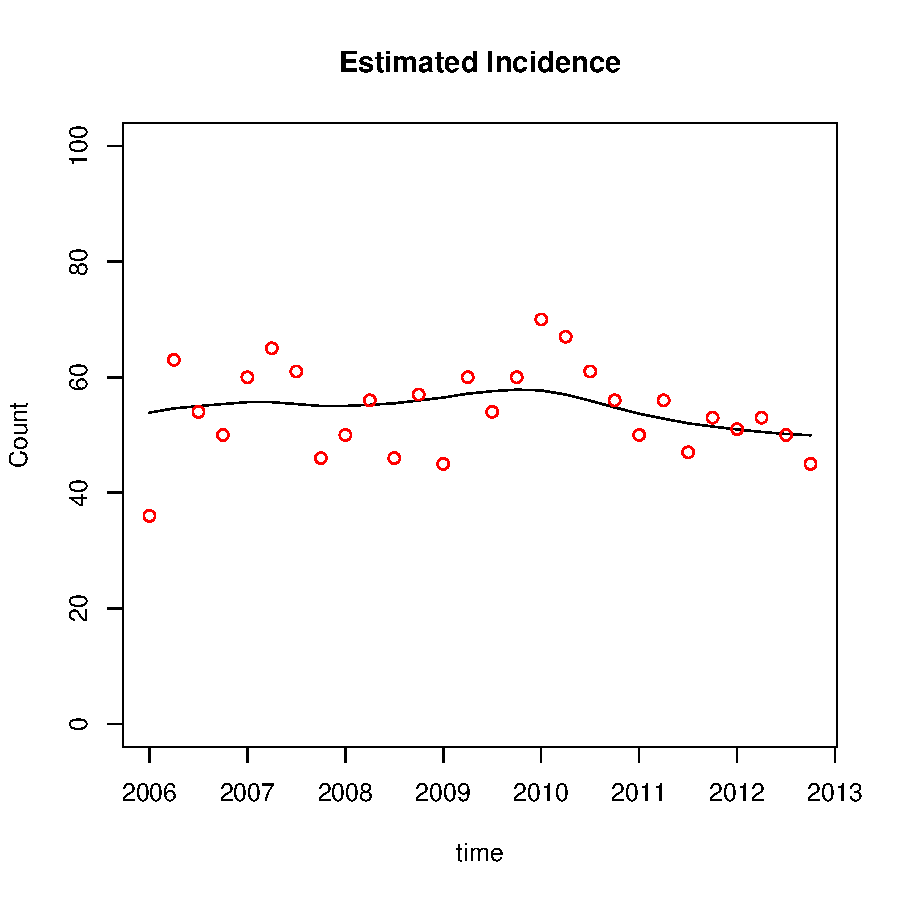
\includegraphics{analysis-002}
This indicates a steady rate of infection over the 2006 to 2012 period, with approximatly 55 individuals being infected each quarter.

Next we estiamte the counts of infected individuals who are undiagnosed.
\begin{Schunk}
\begin{Sinput}
> undiag <- estimateUndiagnosed(mod)
> time <- c(2006,2012.75)
> time <- seq(from=time[1],to=time[2],length.out=sum(obs))
> plot(time,undiag[obs],ylim=c(300,500),type="l",
+      main="Undiagnosed Counts",xlab="time",
+      ylab="# of undiagnosed HIV+ Individuals")
\end{Sinput}
\end{Schunk}
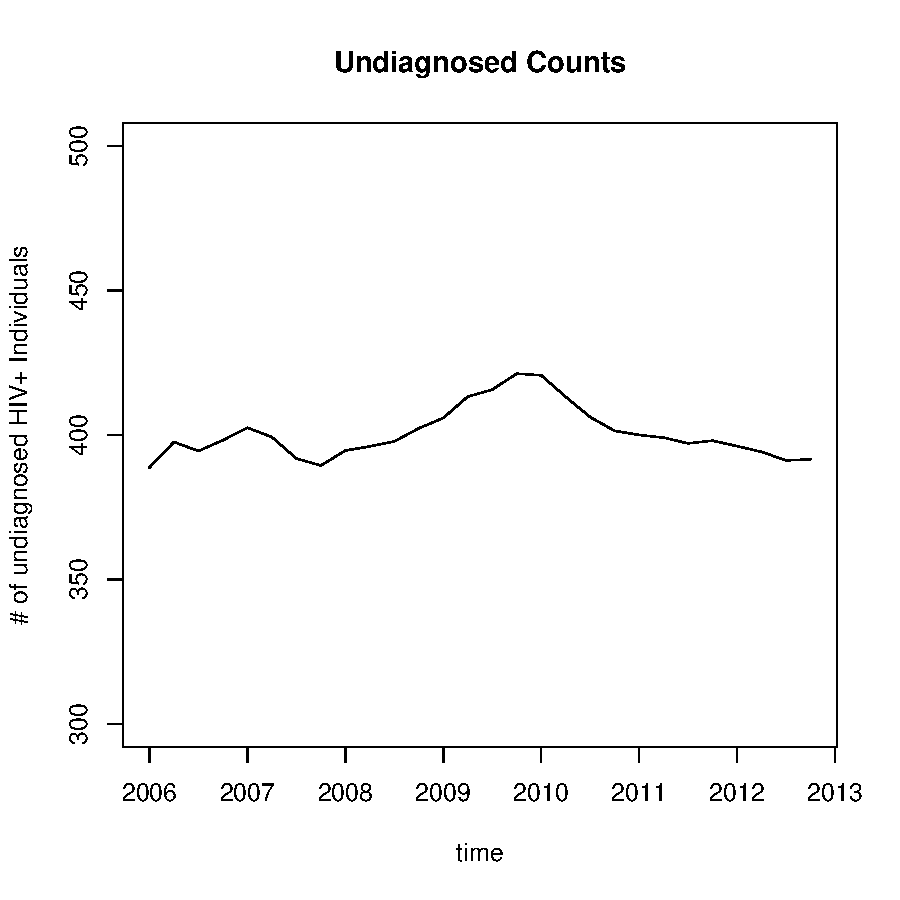
\includegraphics{analysis-003}

Finally we compare to the naive method. The naive method is to multiply incedence times average time to infection. Assuming random infections during the time between last test and diagnosis, the average time from infection to diagnosis in years is:
\begin{Schunk}
\begin{Sinput}
> ti <- with(msm,sort(infPeriod[!is.na(infPeriod) & infPeriod>0]))
> mean(ti/2)
\end{Sinput}
\begin{Soutput}
[1] 1.851559
\end{Soutput}
\end{Schunk}
which, accoarding tot the formula that we were given, leads to an estimate of
\begin{Schunk}
\begin{Sinput}
> incidence <- mean(y,na.rm=TRUE)
> incidence * mean(ti/2)*12/3
\end{Sinput}
\begin{Soutput}
[1] 402.5819
\end{Soutput}
\end{Schunk}

However, though this is in the right ballpark, I can't seem to derive a theoretical basis for its use. If we assume that tehre are no changes in incidence, then the diagnosis counts are estimates of the incidence counts, and the number of undiagnosed infections can be estimated with 
$$
\lim_{j \to \infty} y \sum_{i=0}^jP(D > j-i)
$$
where $y$ is the rate of infection, and $D$ is a random variable representing the probability that someone infected with HIV waits $D$ time intervals before being diagnosed. Using quarterly discrete time units, this yields
\begin{Schunk}
\begin{Sinput}
> j <- 1000
> z <- 0
> for(i in 1:j) z <- z + sum(pid((j-i+1):2000)) + .5*pid(j-i)
> z*incidence
\end{Sinput}
\begin{Soutput}
[1] 408.5285
\end{Soutput}
\end{Schunk}
which is consistant with our model based estimates, as the incidence did not drastically change.

Using the continuous time empirical distribution, and again assuming constant incidence, we get the following estimate for undiagnosed
\begin{Schunk}
\begin{Sinput}
> #continuous density of time between infection and diagnosis
> pi <- function(i){
+   sapply(i,function(ii){
+     ints <- ti[ti>=ii]
+     sum(1/ints)/length(ti)
+   })
+ }
> uti <- unique(ti)
> p<-pi(uti) * diff(c(0,uti))
> cs <- cumsum(p)
> #cdf of density
> qi <- function(u){
+   uind <- rev(which(uti<=u))[1]
+   if(is.na(uind))
+     return(0)
+   cs[uind]
+ }
> n <- 10000
> m <- max(ti)
> s <- seq(from=0,to=m,length.out=n)
> l <- length(ti)
> v <- sum(sapply(s,function(x) (sum(1-qi(x)))))
> v * 4 * incidence / (n/m)
\end{Sinput}
\begin{Soutput}
[1] 408.0196
\end{Soutput}
\end{Schunk}





\end{document}
